\documentclass[11pt]{beamer}
\usepackage{graphicx}
\graphicspath{ {./Images/} }
\setbeamertemplate{caption}[numbered]
\usepackage{caption}
\usepackage{float}
\usepackage{hyperref}
\usepackage{multirow}
\setbeamersize{text margin left=0.5cm,text margin right=0.5cm}
\usepackage{multicol}
\usepackage{listings}
\usepackage{color}
\usepackage{fancyvrb}
\usepackage{booktabs}
\definecolor{dkgreen}{rgb}{0,0.6,0}
\definecolor{gray}{rgb}{0.5,0.5,0.5}
\definecolor{mauve}{rgb}{0.58,0,0.82}
\lstset{
  language=Java,
  aboveskip=3mm,
  belowskip=3mm,
  showstringspaces=false,
  columns=flexible,
  basicstyle={\small\ttfamily},
  numbers=none,
  numberstyle=\tiny\color{gray},
  keywordstyle=\color{blue},
  commentstyle=\color{dkgreen},
  stringstyle=\color{mauve},
  breaklines=true,
  breakatwhitespace=true,
  tabsize=3
}

\makeatletter
\let\save@measuring@true\measuring@true
\def\measuring@true{%
  \save@measuring@true
  \def\beamer@sortzero##1{\beamer@ifnextcharospec{\beamer@sortzeroread{##1}}{}}%
  \def\beamer@sortzeroread##1<##2>{}%
  \def\beamer@finalnospec{}%
}
\makeatother
\mode<presentation> {
    \usetheme{Warsaw}
    \setbeamertemplate{footline}[page number]
    }
\definecolor{violet}{rgb}{0.54, 0.17, 0.89}
\newcommand{\red}[1]{\textcolor{red}{#1}}
\newcommand{\violet}[1]{\textcolor{violet}{#1}}
\newcommand{\green}[1]{\textcolor{green}{#1}}
\newcommand{\sol}{\textbf{Solution}: \pause \newline}

\title[Chapter 03 Notes]{Math 130: Introduction to Programming \\ Chapter 03: Decision Structures \\ Lecture Notes}
\author{Jesús R. Pérez Cuarenta \\
\href{mailto:jperezcuarenta@swccd.edu}{jperezcuarenta@swccd.edu}
}
\date{}

\begin{document}
\section{}
\begin{frame}
  \maketitle
\end{frame}

\begin{frame}
\frametitle{Overview}
    \begin{multicols}{2}
    \tableofcontents
    \end{multicols}
\end{frame}

\section{if, if-else, Nested if Statements}
\subsection{if Statement}
\begin{frame}{if Statement}
    The \violet{if} Statement:
        \begin{center}
        The \violet{if} statement is used to create a decision structure, which allows a program to have more than one path of execution. The \violet{if} statement causes one or more statements to execute only when a \violet{boolean} expression is \violet{true}.
        \end{center}
\end{frame}

\begin{frame}{if Statement}
    So far, programs have been sequentially executed:
        \noindent 
        \begin{figure}[H]
        \centering
        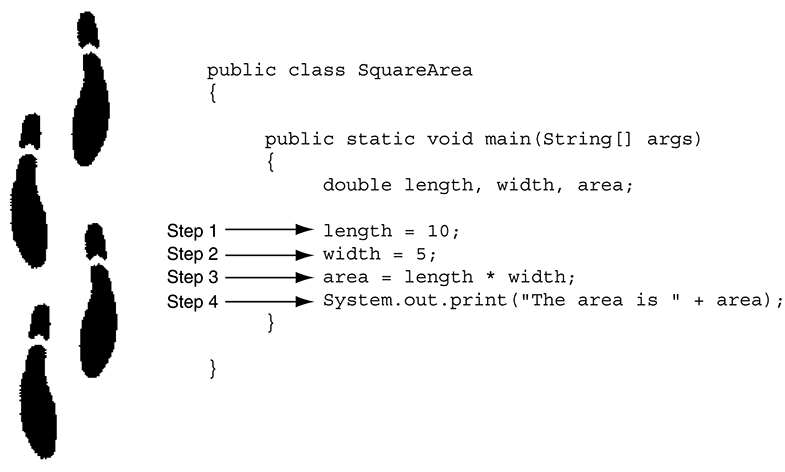
\includegraphics[scale=0.35]{Images/chapter03_sequentialCode.png}
        \end{figure}
\end{frame}

\begin{frame}{if Statement}
    We will now consider programs that execute statements only under certain circumstances. Rather than a sequence structure, we follow a \violet{decision structure}.    
        \noindent 
        \begin{figure}[H]
        \centering
        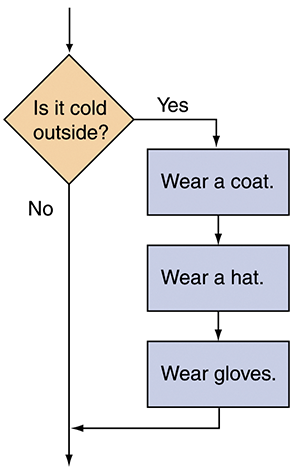
\includegraphics[scale=0.3]{Images/chapter03_decisionCode.png}
        \end{figure}
\end{frame}

\begin{frame}{if Statement}
    The general format will be:
    \vspace{2em}
    \begin{center}
        \noindent \textbf{if} (BooleanExpression) \\ 
        \hspace{1em} statement; 
    \end{center}
    Typically, the \textbf{boolean} expression that is tested by an \textbf{if} statement is formed with a \violet{relational operator}.
\end{frame}

\begin{frame}{Relational Operators}
    \begin{table}[]
    \begin{tabular}{|c|c|}
    \hline
    Relational Operator & Meaning                  \\ \hline
    \textgreater{}      & Greater than             \\ \hline
    \textless{}         & Less than                \\ \hline
    \textgreater{}=     & Greater than or equal to \\ \hline
    \textless{}=        & Less than or equal to    \\ \hline
    ==                  & Equal to                 \\ \hline
    !=                  & Not equal to             \\ \hline
    \end{tabular}
    \end{table}
\end{frame}

\begin{frame}[fragile]{Relational Operators}
    Here is how they look in Java
    \begin{lstlisting}
    // RelationalOperators.java
    public class RelationalOperators {
        public static void main(String[] args) {
            int x, y;
            boolean test1, test2;
            x = 1;
            y = 5;
            test1 = x < y;  // RHS evaluates to true
            test2 = x > y;  // RHS evaluates to false
    
            System.out.println("x < y is: " + test1);
            System.out.println("x > y is: " + test2);
            }
        }
    \end{lstlisting}
\end{frame}

\begin{frame}[fragile]{if Statement with Relational Operator}
    Example code of a relational operator within the \textbf{if} statement call:
    \begin{lstlisting}
    // NumberTest.java
    import java.util.Scanner;
    public class NumberTest {
	   public static void main (String[] args) {
    		Scanner keyboard = new Scanner(System.in);
    		int num;
    		num = keyboard.nextInt();
    		if (num < 0)
    			System.out.println(num + " is negative");
    		else
    			System.out.println(num + " is zero or positive");
    		keyboard.close();
    		}
        }
    \end{lstlisting}
\end{frame}


\begin{frame}[fragile]{Warning}
    Careful with passing semi-colon to if statement after the \textbf{boolean} expression
    \begin{lstlisting}
    // ifStatementWarning.java
    public class ifStatementWarning {
    	public static void main (String[] args) {
    		int x, y;
    		x = 0; 
    		y = 10;
    		if (x > y);	// if statement ends prematurely
    			System.out.print("Statement A");	// always executes
    		if (x > y)	//
    			System.out.print("Statement B");	// executes if x > y
    		}
        }
    \end{lstlisting}
\end{frame}

\subsection{if-else Statement}
\begin{frame}{if-else Statement}
    The \violet{if-else} Statement:
    \begin{center}
        The \violet{if-else} statement will execute one group of statements if its \violet{boolean} expression is \violet{true}, or another group of its \violet{boolean} expression is \violet{false}.
    \end{center}
    In general form: \\

    \noindent
    \textbf{if} (BooleanExpression) \\
    \hspace{1em} statement or block
    \flushleft \textbf{else} \\ 
    \hspace{1em} statement or block
\end{frame}

\begin{frame}[fragile]{if-else Statement}
    Example code with if-else
        \begin{lstlisting}
    // Division.java
    public class Division {
    	public static void main (String[] args) {
    		double number1, number2, quotient;
    		number1 = 10;
    		number2 = 5;
    		if (number2 == 0)
    			System.out.print("Division by zero not allowed.");
    		else {
    			quotient = number1 / number2;
    			System.out.print("Quotient is: " + quotient);
    			}
    		}
        }
    \end{lstlisting}
\end{frame}

\subsection{Nested if Statements}
\begin{frame}{Nested if Statements}
    Nested if Statements:
    \begin{center}
        To test more than one condition, an \violet{if} statement can be nested inside another \violet{if} statement.
    \end{center}

    Example:
    Qualifying for a bank loan with the conditions being (1) customer's salary and (2) customer's job history.
\end{frame}

\begin{frame}{Nested if Statements}
    Use the Scanner class and write a program that aligns with the flow chart.
        \noindent 
        \begin{figure}[H]
        \centering
        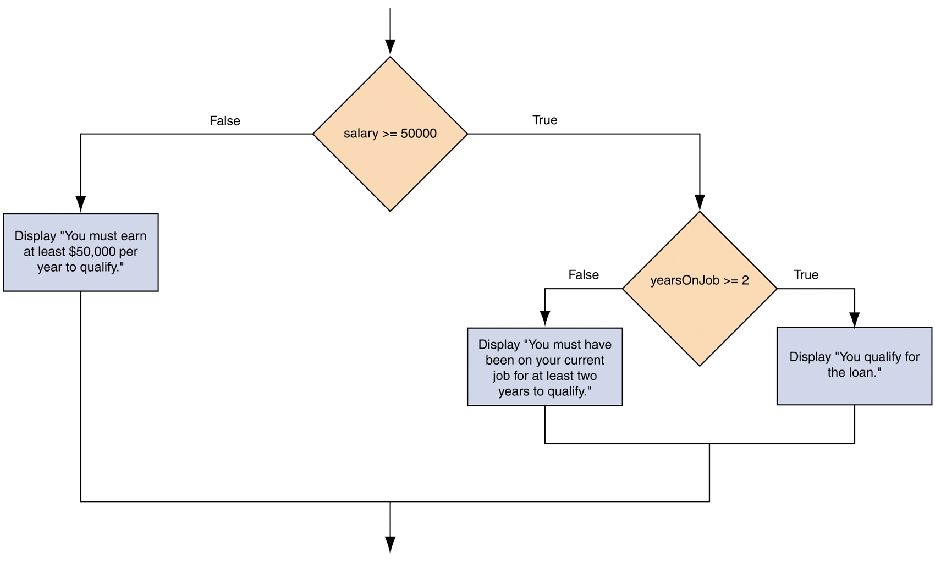
\includegraphics[scale=0.3]{Images/chapter03_nestedIf.png}
        \end{figure}
\end{frame}

\begin{frame}{Nested if Statements}
    Suppose you wanted to write a program that achieves the following.
    \noindent 
    \begin{figure}[H]
    \centering
    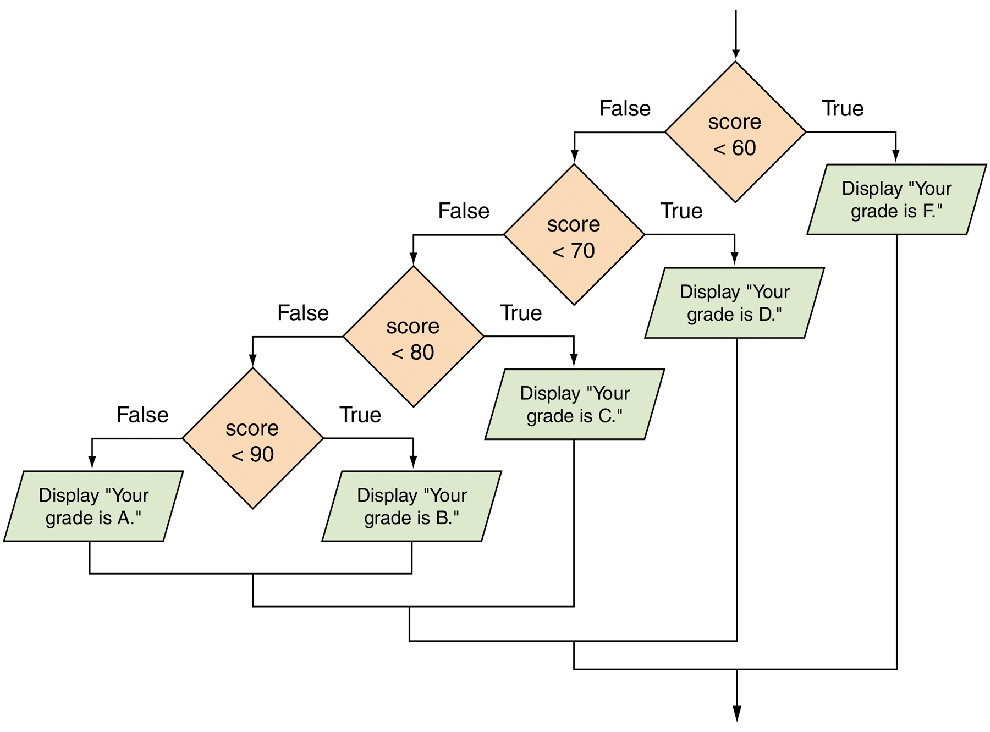
\includegraphics[scale=0.25]{Images/chapter03_nestedIfGradeProgram.png}
    \end{figure}
\end{frame}


\subsection{if-else-if Statement}
\begin{frame}{if-else-if Statement}
    The if-else-if Statement
    \begin{center}
        The \violet{if-else-if} statement tests a series of conditions. It is often simpler to test a series of conditions with the \violet{if-else-if} statement than with a set of nested \violet{if-else} statements.
    \end{center}
\end{frame}

\begin{frame}{if-else-if Statement}
    General idea for \violet{if-else-if}:
    \noindent 
    \begin{figure}[H]
    \centering
    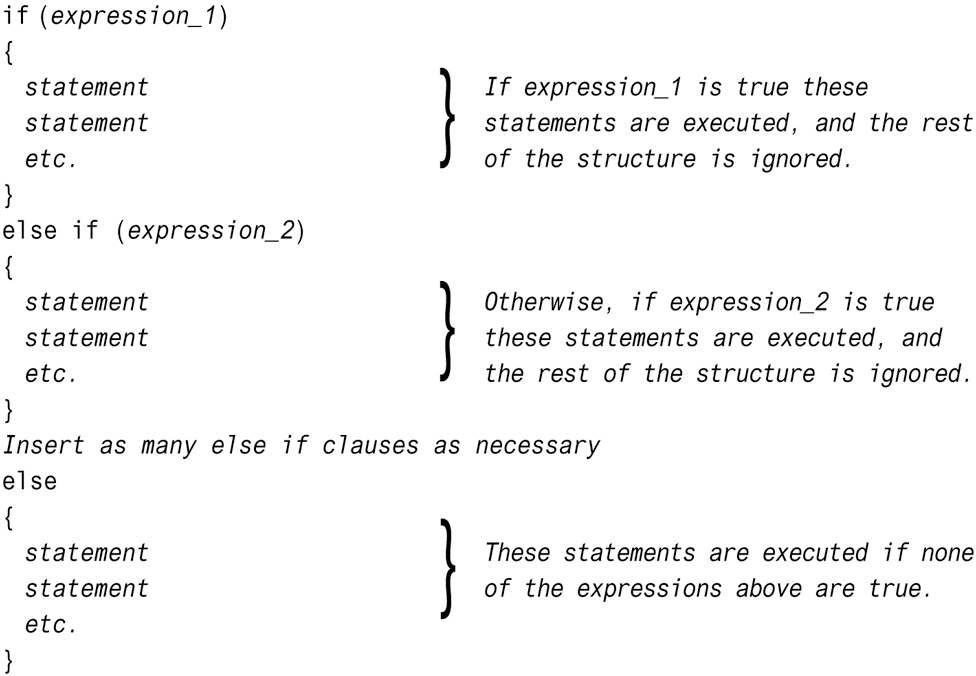
\includegraphics[scale=0.25]{Images/chapter03_ifElseIf.png}
    \end{figure}
\end{frame}

\begin{frame}{if-else-if Statement}
    How would you rewrite this flow chart?
    \noindent 
    \begin{figure}[H]
    \centering
    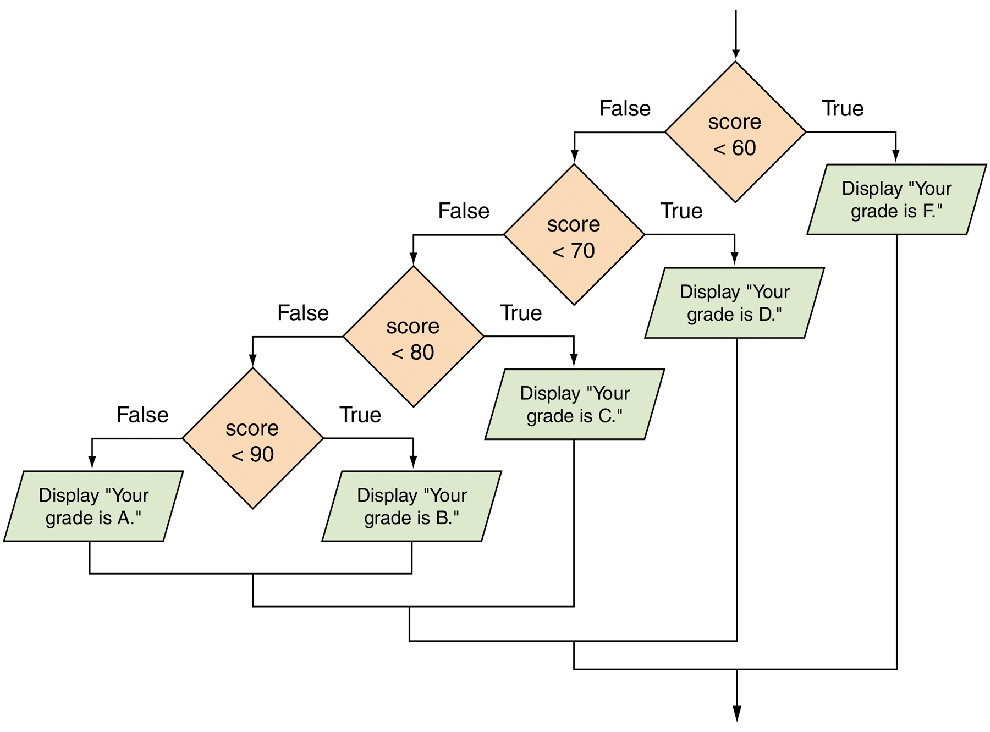
\includegraphics[scale=0.25]{Images/chapter03_nestedIfGradeProgram.png}
    \end{figure}
\end{frame}

\section{Logical Operators}
\subsection{AND, OR, NOT}
\begin{frame}{Logical Operators}
    \begin{center}
        \violet{Logical operators} connect two or more relational expressions into one or reverse the logic of an expresison.
    \end{center}
    Java provides two binary logical operators, \red{\&\&} and \red{$\mid \mid$}, which are used to combine two \violet{boolean} expressions into a single expression. It also provides the unary operator \red{!}, which reverses the truth of a \violet{boolean} expression.
    \vspace{1em}

    Here is a convenient table,
    \begin{table}[]
    \begin{tabular}{|c|c|}
    \hline
    Operator & Meaning \\ \hline
    \&\&     & AND     \\ \hline
    $\mid \mid$        & OR      \\ \hline
    !        & NOT     \\ \hline
    \end{tabular}
    \end{table}
\end{frame}

\begin{frame}[fragile]{Logical Operators - AND}
    Example code with logical operator \&\& 
    \begin{lstlisting}
    // LogicalAnd.java
    public class LogicalAnd {
    	public static void main (String[] args) {
    		double temperature, minutes;
    		temperature = 5;
    		minutes = 20;
    		if (temperature < 20 && minutes > 12)	// AND
    			System.out.print("Danger.");
    		}
        }
    \end{lstlisting}
\end{frame}

\begin{frame}[fragile]{Logical Operators - OR}
    Example code with logical operator $\mid \mid$
    \begin{lstlisting}
    // LogicalOr.java
    public class LogicalOr {
    	public static void main (String[] args) {
    		double temperature;
    		temperature = 120;
    		if (temperature < 20 || temperature > 100)	// OR
    			System.out.print("Danger.");
        }
    \end{lstlisting}
\end{frame}

\begin{frame}[fragile]{Logical Operators - NOT}
    Example code with logical operator !
    \begin{lstlisting}
    // LogicalNot.java
    public class LogicalNot {
    	public static void main (String[] args) {
    		double temperature;
    		temperature = 50;
    		if (!(temperature > 100))	// NOT
    			System.out.print("Danger.");
    		}
        }
    \end{lstlisting}
\end{frame}

\subsection{Precedence}
\begin{frame}{Precedence}
    \begin{table}[]
    \begin{tabular}{|c|c|}
    \hline
    Order of Precedence & Operators                                                  \\ \hline
    1                   & -, !                                                       \\ \hline
    2                   & *, /, \%                                                   \\ \hline
    3                   & +, -                                                       \\ \hline
    4                   & \textless{}, \textgreater{}, \textless{}=, \textgreater{}= \\ \hline
    5                   & ==, !=                                                     \\ \hline
    6                   & \&\&                                                       \\ \hline
    7                   & $\mid \mid$                                                \\ \hline
    8                   & =, +=, -=, *=, \%=                                         \\ \hline
    \end{tabular}
    \end{table}
    Or just use parenthesis \ldots
\end{frame}

\section{Comparing String Objects}
\begin{frame}[fragile]{Comparing String Objects}
    When comparing {String} objects, it is best to do so with String methods.
        \begin{lstlisting}
        String name1 = "Mark";
        String name2 = "Mary";
        if (name1 == name2) { // false
            System.out.print("Something.");
            }
    \end{lstlisting}
    The previous relational operator evaluates to false but not because the strings are different. It's because it's comparing the address of the String objects.
\end{frame}

\subsection{String.equals() Method}
\begin{frame}[fragile]{String.equals() Method}
    We can instead call the String class's \violet{equals} method.
        \begin{lstlisting}
        String name1 = "Mark";
        String name2 = "Mary";
        if (name1.equals(name2)) { // false
            System.out.print("Something.");
            }
    \end{lstlisting}
\end{frame}

\begin{frame}[fragile]{String.equals() Method}
    For those of you that are not convinced, feel free to play around with this example.
        \begin{lstlisting}
        String name1 = "Mark";
        String name2 = "Mark";
        String name3 =  new String("Mark"); 
        System.out.println(name1 == name2); // true
        System.out.println(name1 == name3); // false
        System.out.println(name1.equals(name2)); // true
        System.out.println(name1.equals(name3)); // true
        \end{lstlisting}
\end{frame}

\subsection{Other String Methods}
\begin{frame}[fragile]{String.compareTo() Method}
    \begin{itemize}
        \item
            The \violet{compareTo} method can be used to determine whether one string is greater than, equal to, or less than another string.
        \item
            The \violet{equalsIgnoreCase} method behaves like \violet{String.equals()} but ignores the case of the characters in the strings.
        \item
            The \violet{compareToIgnoreCase} method behaves like \violet{compareTo} but ignores the case of the characters in the strings.
    \end{itemize}
\end{frame}

\section{Scope, Conditional Operator, switch, and Formatted Output}
\subsection{Scope}
    
\begin{frame}{Scope}
    The \violet{scope} of a variable is limited to the block in which it is declared. \\
    \vspace{1em}
    A variable's \violet{scope} is the part of the program where the variable's name may be used. \\
    \vspace{1em}
    A local variable's \violet{scope} always starts at the variable's declaration, and ends at the closing brace of the block of code in which it is declared in.
\end{frame}

\subsection{Conditional Operator}
\begin{frame}{The Conditional Operator}
    You can use the conditional operator to create short expressions that work like \violet{if-else} statements. \\
    \vspace{1em}
    Because it takes three operands, it is considered a ternary operator. \\
    \vspace{1em}
    The operator consists of a question mark (\red{?}) and a colon (\red{:}). \\
    \vspace{1em}
    General form: \\
    BooleanExpression ? Value1 : Value 2
\end{frame}

\begin{frame}[fragile]{Numeric Example}
    The following code showcases how to interchange if-else with conditional operators on numeric data.
    \begin{lstlisting}
        // if-else
        if (x < 0)
            y = 10;
        else
            y = 20;
        // Conditional operator
        y = x < 0 ? 10 : 20;
    \end{lstlisting}
\end{frame}

\begin{frame}[fragile]{Printing String Object Example}
    The following code showcases how to interchange if-else with conditional operators on String objects.
    \begin{lstlisting}
        // if-else
        if (score < 60)
            System.out.println("Your grade is: Fail");
        else
            System.out.println("Your grade is: Pass");
        // Conditional operator
            System.out.println("Your grade is " 
                + (score < 60 ? "Fail." : "Pass.")
                );
    \end{lstlisting}
\end{frame}

\subsection{switch Statement}
\begin{frame}{switch Definition and Examples}
    The \violet{switch} statement lets the value of a variable or expression determine where the program will branch to.
\end{frame}

\begin{frame}{The switch Statement}
    \noindent 
    \begin{figure}[H]
    \centering
    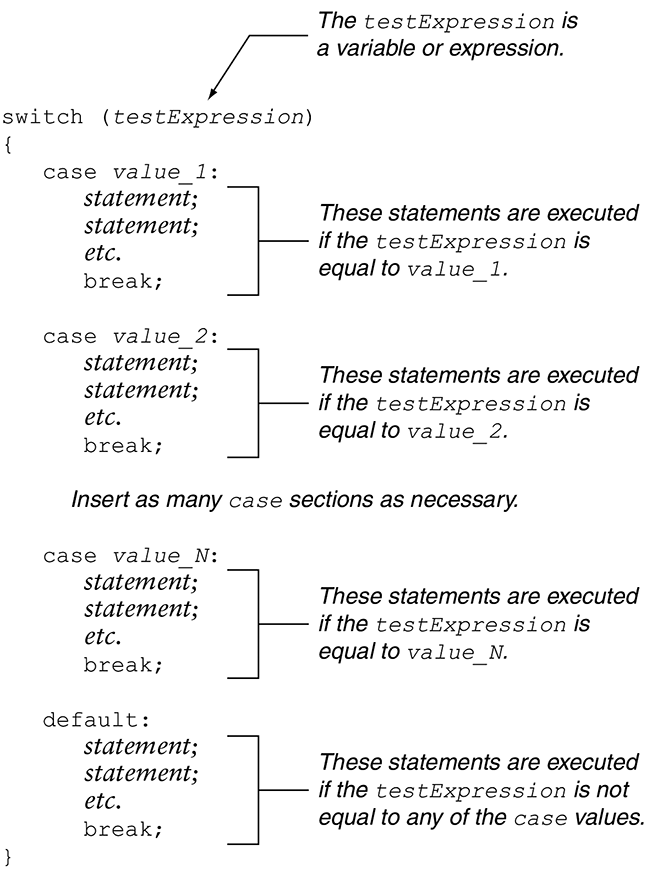
\includegraphics[scale=0.2]{Images/chapter03_switchStatement.png}
    \end{figure}
\end{frame}


\begin{frame}[fragile]{switch Example}
    Assume \violet{month} is an \violet{int} variable.
    \begin{lstlisting}
    switch (month) {
        case 1:
            System.out.println("January");
            break;
        case 2:
            System.out.println("February");
            break;
        case 3:
            System.out.println("March");
            break;
        default:
            System.out.println("Other");
            break;
            }
    \end{lstlisting}
\end{frame}

\begin{frame}[fragile]{switch Example}
    Here is the previous example in terms of if-else statements.
    \begin{lstlisting}
    if (month == 1)
        System.out.println("January");
    else if (month == 2)
        System.out.println("February");
    else if (month == 3)
        System.out.println("March");
    else
        System.out.println("Other");
    \end{lstlisting}
\end{frame}

\begin{frame}[fragile]{switch Example}
    Multi Value case Statements (Java 12 and Later) example
    \begin{lstlisting}
    switch (month) {
        case 1, 2, 3, 4, 5:
            System.out.println("Spring Semester");
            break;
        case 6, 7:
            System.out.println("Summer Semester");
            break;
        case 8, 9, 10, 11, 12:
            System.out.println("Fall Semester");
            break;
        default:
            System.out.println("Error: Invalid month");
        }
    \end{lstlisting}
\end{frame}

\subsection{Formatted Output}
\begin{frame}{Formatted Output}
    The \violet{System.out.printf} method allows you to format output in a variety of ways. The \violet{String.format} method allows you to format a string, without displaying it. The string can be displayed at a later time.
\end{frame}

\begin{frame}[fragile]{Formatted Output}
    Old way:
    \begin{lstlisting}
    double number = 10.0 / 6.0;
    System.out.println(number);
    \end{lstlisting}

    Alternative way:
    \begin{lstlisting}
    double sales = 12345.67;
    System.out.printf("Our sales are %f for the day.", sales);
    \end{lstlisting}

    We call \violet{\%f} a format specifier indicating floating-point value insertion. It can be used with \violet{float} or \violet{double} arguments.
\end{frame}

\begin{frame}[fragile]{Formatted Output}
    We can also pass several arguments:
    \begin{lstlisting}
    double value1 = 3.0;
    double value2 = 6.0;
    double value3 = 9.0;
    System.out.printf("%f %f %f", value1, value2, value3);
    \end{lstlisting}

    There is another format specifier, \violet{\%d}, which stands for decimal integer. It can be used with arguments of the \violet{int, short, and long} data types.

    \begin{lstlisting}
    int dogs = 2;
    int cats = 4;
    System.out.printf("%d dogs and %d cats.", dogs, cats);
    \end{lstlisting}    
\end{frame}

\begin{frame}[fragile]{Formatted Output}
    Precision is given by specifying decimal places:
    \begin{lstlisting}
    double temp = 78.42819;
    System.out.printf("The temperature is %.2f degrees.", temp);
    \end{lstlisting}
    And similarly,
    \begin{lstlisting}
    double value1 = 123.45678;
    double value2 = 123.45678;
    double value3 = 123.45678;
    System.out.printf("%.1f %.2f %.3f", value1, value2, value3);            
    \end{lstlisting}
\end{frame}

\begin{frame}[fragile]{Formatted Output}
    Here is an example of the \violet{String.format} method:
    \begin{lstlisting}
public class CurrencyFormat2 {
    public static void main(String[] args) {
    double monthlyPay = 5000.0;
    double annualPay = 12 * monthlyPay;

    String output = String.format("Pay is $%,.2f\n", annualPay);
    System.out.println(output);
    }
}
    \end{lstlisting}
\end{frame}

\end{document}

